\documentclass[11pt]{article}
\usepackage[preprint]{acl}
\usepackage{times}
\usepackage{latexsym}
\usepackage[T1]{fontenc}
\usepackage[utf8]{inputenc}
\usepackage[expansion=false]{microtype}
\usepackage{amsmath,amssymb}
\usepackage{booktabs}
\usepackage{graphicx}
\usepackage{xcolor}
\graphicspath{{figures/}}

\newcommand{\goldtwo}{\textsc{gold@}$2$}
\newcommand{\sm}{\textsc{SpikeMem}}

\title{\sm: A Spiking Associative Memory for Multi-Hop Question Answering\\
over Updated Facts in LLM Agents}

\author{
  Shiteng Lu \and Malu Zhang \\
  Yingcai Honors College, University of Electronic Science and Technology of China
}

\begin{document}
\maketitle

\begin{abstract}
Agent memories must answer multi-hop questions over facts that change: a bridge entity may have
been superseded, and the signal that it was superseded may itself be missing or wrong. We present
\sm{}, an associative memory built from leaky integrate-and-fire fact units in which three
computations are expressed as circuit motifs: a coincidence threshold gates each hop on subject and
relation jointly, conduction delays count hops, and winner-take-all slot competition with directed,
finite supersede inhibition arbitrates between versions before activity propagates. The circuit
returns a single winning evidence chain, which the downstream reader can read out without a pairwise
decision. On a MuSiQue-derived benchmark with superseded bridge entities and ten settings of
update-evidence noise, evaluated end to end with a frozen Qwen3-8B reader and order-balanced scoring,
\sm{} ties a one-shot temporal knowledge-graph memory on clean data and exceeds both its hard- and
soft-invalidation variants in all nine noisy settings, by up to $+0.138$ exact match, while losing
only $0.048$ from clean to the strongest noise. Analysis attributes the margin to three design
properties: hop-by-hop search reaches updated bridges that a one-shot pool misses, finite inhibition
keeps falsely expired facts recoverable, and single-winner read-out avoids an order-sensitive reader
decision. \sm{}'s dynamics compile to an equivalent event-driven graph search, so these gains reflect
the computations the circuit performs rather than spike timing as such.
\end{abstract}

% =====================================================================
\section{Introduction}

Long-lived language agents accumulate facts that change. A user moves, a company changes its CEO,
a document is revised. Answering a multi-hop question such as ``Which country is the current
employer of X's spouse based in?'' then requires two things at every hop: finding the fact that links
the current entity to the next, and choosing the \emph{current} version when several versions of that
fact are stored. Agent memory systems address the second requirement with add/update/delete
operations \citep{chhikara2025mem0} or temporally scoped graph edges \citep{rasmussen2025zep}, but in
deployment the evidence that one fact supersedes another is itself inferred, and can be missing (a
stale fact still looks current) or spurious (a current fact looks expired).

Neural circuits face a structurally similar problem---selecting one interpretation among competing,
partially reliable inputs---and solve it with a small set of motifs: coincidence detection,
conduction delay, lateral inhibition, and winner-take-all competition
\citep{shastri1993shruti,maass2000wta}. \sm{} uses these motifs as the design language for an agent
memory. Each stored fact is a leaky integrate-and-fire (LIF) unit. A fact fires only when its subject
and relation are activated together, so each hop is a conjunction; conduction delays place the $k$-th
hop at a known time, so hop depth needs no explicit counter; and facts that fill the same
(subject, relation) slot compete, with newer versions inhibiting older ones through edges written at
insertion time. Because inhibition is finite rather than masking, a fact wrongly marked as expired
can still win when it is the only candidate that completes the chain.

The circuit settles on a single winning chain. This matters downstream in a way we did not initially
anticipate: a single chain can be read out directly, whereas a memory that returns two candidate
chains forces the reader into a pairwise decision that, for current LLM readers, is strongly
order-sensitive \citep{wang2024fair,zheng2023judge}. Section~\ref{sec:analysis} quantifies this.

\paragraph{Contributions.}
(1) \sm{}, an agent memory in which conjunctive hop gating, hop counting, and version arbitration are
implemented as spiking circuit motifs with write-time supersede inhibition (\S\ref{sec:method}).
(2) An end-to-end evaluation on multi-hop questions with superseded bridge entities, ten settings of
update-evidence noise, and a sweep over update prevalence, against temporal knowledge-graph and
graph-propagation memories that share one frozen reader and an order-balanced protocol
(\S\ref{sec:setup}, \S\ref{sec:results}). (3) An analysis that decomposes \sm{}'s margin into search
reach, recoverable inhibition, and single-winner read-out, including a controlled intervention on the
read-out (\S\ref{sec:analysis}).

% =====================================================================
\section{Related work}

\paragraph{Agent memory under updates.}
Mem0 \citep{chhikara2025mem0} maintains memory through LLM-issued add, update, and delete operations;
Zep \citep{rasmussen2025zep} stores temporally scoped knowledge-graph edges; LongMemEval
\citep{wu2025longmemeval} and MemoryAgentBench \citep{hu2026memoryagentbench} evaluate knowledge
updates, and \citet{yadav2026temporal} show that retaining superseded history without supersession is
severely damaging. Temporal knowledge-graph QA answers multi-hop questions over time-stamped facts
\citep{saxena2021cronkgqa}. \sm{} differs in performing arbitration inside the retrieval dynamics, hop
by hop, and in tolerating noisy supersession evidence through finite inhibition.

\paragraph{Multi-hop retrieval.}
Iterative retrieve-and-reason interleaves retrieval with chain-of-thought
\citep{trivedi2023interleaving,press2023measuring}; HippoRAG applies personalized PageRank over an
entity graph \citep{gutierrez2024hipporag}, which we include as a baseline.

\paragraph{Spiking associative memory.}
Temporal synchrony for variable binding originates with \citet{shastri1993shruti}; winner-take-all
computation and spike-timing plasticity are classical \citep{maass2000wta,caporale2008stdp}. We claim
no novelty for these components; the contribution is their composition into an agent memory for
multi-hop reasoning over updated facts. Spiking graph algorithms have provable advantages in
neuromorphic hardware cost models \citep{aimone2020neuromorphic}; we do not evaluate on such hardware.

\paragraph{Reader-side position bias.}
LLM judges and readers prefer candidates by position, and fair comparison requires evaluating both
orders \citep{wang2024fair,zheng2023judge,shi2024judges}. More retrieved context can also hurt
\citep{hsia2024ragged,cuconasu2024noise}. We adopt order-balanced scoring throughout, and
\S\ref{sec:analysis} shows why it matters for comparing memories.

% =====================================================================
\section{\sm}
\label{sec:method}

\begin{figure}[t]
\centering
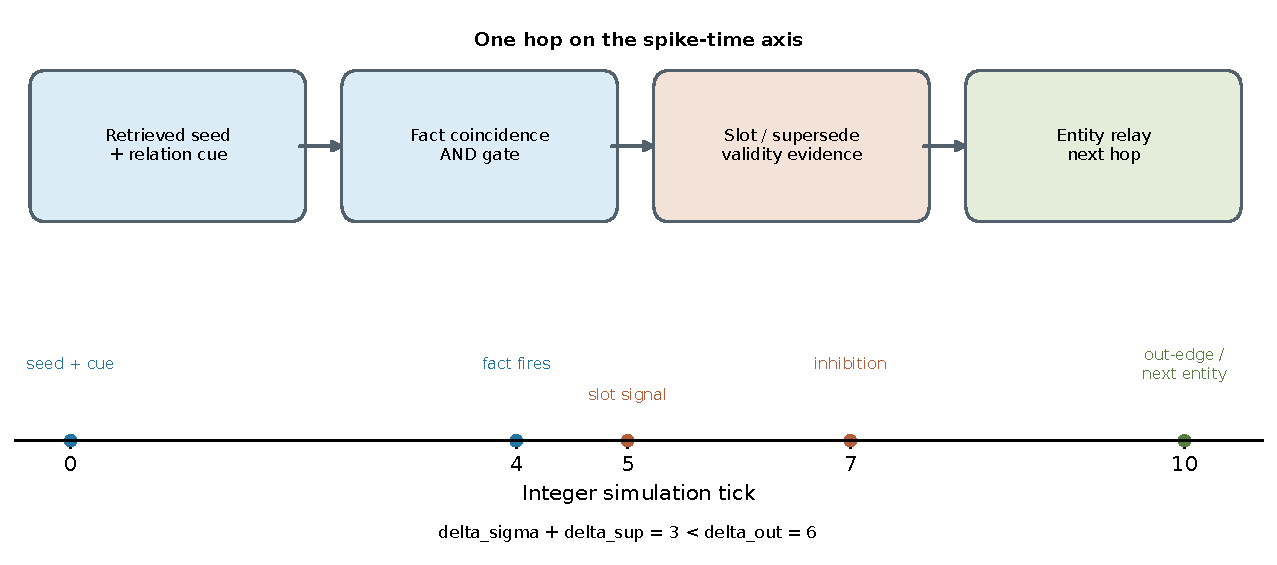
\includegraphics[width=\columnwidth]{fig1_architecture_timing.pdf}
\caption{\sm{} expresses three computations on one time axis: conduction delay $\delta_h$ counts
hops, coincidence under $A<\theta<2A$ binds subject and relation, and slot competition with directed
supersede inhibition arbitrates, with $\delta_\sigma+\delta_{\text{sup}}<\delta_{\text{out}}$ so a
superseded fact is suppressed before its outgoing edge fires.}
\label{fig:arch}
\end{figure}

\paragraph{Memory representation.}
Memory is a graph of localist fact units $m_i=(s_i,p_i,v_i,d_i,c_i,z_i)$: subject, predicate, value,
write order, confidence, and validity state. When a write $s\xrightarrow{p}v_{\text{new}}$ fills a
slot $\sigma=(s,p)$ already holding $v_{\text{old}}$, a directed supersede edge from the new unit to
the old one is created at write time. Direction is taken from the write stream because read-time
co-activation is symmetric and cannot identify which version is newer.

\paragraph{Dynamics.}
Each fact unit is a leaky integrate-and-fire neuron,
\begin{align}
V_i(t) = {}& \beta V_i(t-1) + \alpha\,g(q,m_i) \nonumber\\
 & + \textstyle\sum_j w_{ij}\,s_j(t-\delta_{ij}) \nonumber\\
 & - \textstyle\sum_j \mu_{ij}\,s_j(t-\delta_{\text{sup}}),
\end{align}
firing when $V_i(t)\ge\theta_i$, where $g(q,m_i)$ is query similarity, $w_{ij}$ are excitatory edges
from upstream facts, and $\mu_{ij}$ are supersede inhibitions.

\paragraph{Conjunctive hop gating.}
With single-input postsynaptic peak $A$ and $A<\theta_i<2A$, no single input fires a unit: subject and
relation activation must coincide within $\tau_c=\ln(\theta_i/A-1)/\ln\beta$, which is positive
because numerator and denominator are both negative. Each hop is thus an AND over subject and
relation, which rejects facts that match only one of them.

\paragraph{Hop counting.}
A per-hop conduction delay $\delta_h$ places hop-$k$ facts near $k\delta_h$, so a read-out window
selects chains of the decomposed length and rejects under-length shortcuts.

\paragraph{Version arbitration.}
Facts in the same slot compete through a winner-take-all slot node, and supersede edges inhibit older
versions. The timing constraint $\delta_\sigma+\delta_{\text{sup}}<\delta_{\text{out}}$ ensures that a
superseded fact is suppressed \emph{before} its outgoing edge excites the next hop, so arbitration
happens before propagation rather than after. Inhibition is finite: a falsely expired fact is
weakened, not removed, and can still win if it is the only candidate that completes the chain.

\paragraph{Single-winner read-out.}
The first chain to complete within the hop window is returned. Because arbitration has already
selected one version per slot, the memory returns a single chain, whose terminal value is read out
directly; the reader adjudicates only when more than one chain survives.

\paragraph{Implementation.}
We simulate the network with an event-driven scheduler. The same computations can be executed as an
event-driven graph search with an explicit AND filter, hop counter, and sparse arbitration; on all
$24{,}170$ query--setting pairs of our evaluation this produces identical outputs. We therefore
attribute \sm{}'s behaviour to the computations its circuit performs rather than to spike timing as
such, and regard the spiking form as the design language and an implementation suited to
event-driven hardware, which we do not evaluate here.

% =====================================================================
\section{Experimental setup}
\label{sec:setup}

\paragraph{Benchmark.}
We adapt the $2{,}417$ answerable questions of the MuSiQue development split
\citep{trivedi2022musique}, whose per-hop decompositions give full gold chains of length
$K\in\{2,3,4\}$ without entity-recognition heuristics. With probability $\rho$ ($0.5$ unless stated)
a bridge slot is updated: an old value, drawn from a genuine MuSiQue distractor title rather than
synthesised, is written before the new one, and the gold chain continues from the new value.

\paragraph{Update-evidence noise.}
Supersede evidence is corrupted in two ways at rates $0.1$, $0.2$, and $0.3$: \emph{false positive}
(\textsc{fp}), a valid fact is marked expired; \emph{false negative} (\textsc{fn}), a real supersede
edge is dropped so that stale and current versions both appear valid. Three diagonal settings
($\textsc{fp}=\textsc{fn}$) and a clean setting give ten configurations. Injection and noise are
query-scoped, and we verified that neither leaks across questions nor destroys chains by construction
(Appendix~\ref{sec:selfchecks}).

\paragraph{Entry.}
All methods enter the graph with the same sparse TF--IDF retriever over the question and entity
titles, using no gold seed, answer, path, or support annotation (full-dev seed@1 $=0.6856$).

\paragraph{Reader and scoring.}
A frozen Qwen3-8B reader (greedy decoding, non-thinking mode, at most 16 new tokens) sees the question
and the rendered candidate chains with write orders, and may answer \texttt{INSUFFICIENT}; it never
sees gold labels or noise types. A single candidate chain is read out directly. Every two-candidate
decision is run in both presentation orders and scored as the mean of the two correctness indicators
\citep{wang2024fair,zheng2023judge}. Reader calls are deterministically cached, with zero parse
failures. Differences use a paired bootstrap over questions with $2{,}000$ resamples.

\paragraph{Baselines.}
All methods share the graph, entry retriever, reader, and prompt template.
\emph{Temporal KG (hard / soft)}: one-shot search over a temporally scoped graph in the style of
\citet{rasmussen2025zep}, with hard invalidation (expired facts removed) or soft invalidation (expired
facts down-weighted), enumerating up to two complete chains from a top-16 pool.
\emph{Personalized PageRank}: sparse PPR over the fact graph in the style of
\citet{gutierrez2024hipporag}.

% =====================================================================
\section{Results}
\label{sec:results}

\begin{table*}[t]
\centering
\caption{Order-balanced exact match on MuSiQue full-dev ($N=2{,}417$), text entry, $\rho=0.5$,
temporal top-16. $\Delta$ columns are \sm{} minus each baseline. Bold marks the best method per row.}
\label{tab:main}
\small
\begin{tabular}{lrrrrr}
\toprule
Noise & TKG hard & TKG soft & \sm{} & $\Delta$ hard & $\Delta$ soft \\
\midrule
clean            & \textbf{.6856} & .6243 & \textbf{.6856} & $.0000$  & $+.0612$ \\
\textsc{fp}$=.1$ & .6347 & .6055 & \textbf{.6756} & $+.0410$ & $+.0701$ \\
\textsc{fp}$=.2$ & .5925 & .5904 & \textbf{.6663} & $+.0739$ & $+.0759$ \\
\textsc{fp}$=.3$ & .5445 & .5770 & \textbf{.6566} & $+.1121$ & $+.0796$ \\
\textsc{fn}$=.1$ & .6756 & .6229 & \textbf{.6769} & $+.0012$ & $+.0540$ \\
\textsc{fn}$=.2$ & .6663 & .6202 & \textbf{.6709} & $+.0046$ & $+.0507$ \\
\textsc{fn}$=.3$ & .6566 & .6171 & \textbf{.6651} & $+.0085$ & $+.0480$ \\
diag $=.1$       & .6309 & .6057 & \textbf{.6696} & $+.0387$ & $+.0639$ \\
diag $=.2$       & .5662 & .5896 & \textbf{.6560} & $+.0898$ & $+.0664$ \\
diag $=.3$       & .5002 & .5577 & \textbf{.6380} & $+.1378$ & $+.0803$ \\
\bottomrule
\end{tabular}
\end{table*}

\subsection{Accuracy under update noise}

Table~\ref{tab:main} gives end-to-end accuracy. \sm{} ties hard invalidation on clean data and leads
both temporal-KG variants in all nine noisy settings, by up to $+0.138$ over hard invalidation
(diagonal $0.3$) and up to $+0.080$ over soft invalidation. The margins over hard invalidation are
large under false-positive noise ($+0.041$ to $+0.112$) and small under false-negative noise
($+0.001$ to $+0.009$), which is what the design predicts: a falsely expired gold fact is deleted by
hard invalidation but only weakened by \sm{}'s finite inhibition, whereas a dropped supersede edge
removes the information both methods would need.

\sm{} also degrades most gracefully. From clean to diagonal $0.3$ it loses $0.048$, against $0.185$
for hard and $0.067$ for soft invalidation. The two invalidation policies cross: hard is better on
clean and \textsc{fn} data, soft under strong \textsc{fp} noise, because soft retains falsely expired
gold facts but returns extra candidate chains that cost accuracy at the reader (\S\ref{sec:analysis}).
\sm{} does not face this trade-off: it retains the falsely expired fact and still returns one chain.

Personalized PageRank is not competitive in this setting. On clean full-dev it reaches $0.00745$ exact
match while performing about $6{,}363$ sparse edge relaxations per query; \sm{} reaches $0.68556$ with
$27.9$ edge accesses per query. Both counts are work proxies within our implementation rather than
calibrated costs, and the gap reflects that single-pass diffusion followed by top-$k$ ranking does not
enforce the per-hop conjunctions these questions require.

\begin{figure}[t]
\centering
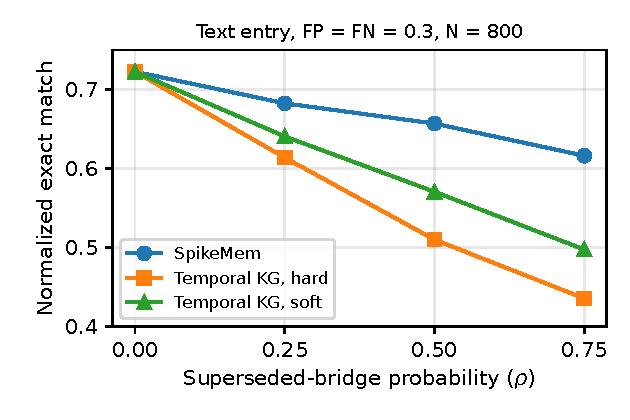
\includegraphics[width=\columnwidth]{fig3_rho_scan.pdf}
\caption{Order-balanced exact match as the prevalence $\rho$ of superseded bridge entities varies
($\textsc{fp}=\textsc{fn}=0.3$, text entry, $N=800$). Rebuilding the graph at each $\rho$ also changes
entry difficulty (seed@1 moves from $0.7225$ at $\rho=0$ to $0.7000$ at $\rho=0.75$), so we compare
methods within each $\rho$ rather than reading the absolute slope.}
\label{fig:rho}
\end{figure}

\subsection{Prevalence of updates}

Figure~\ref{fig:rho} varies the fraction of updated bridge slots under combined noise. All methods
coincide at $\rho=0$, where there is nothing to arbitrate, and the gap between \sm{} and both
temporal-KG variants widens as updates become more common, with hard invalidation falling fastest.
The benefit of in-search arbitration therefore grows with the rate at which memory changes.

% =====================================================================
\section{Where the margin comes from}
\label{sec:analysis}

To understand the margin, we take its largest robust instance, \textsc{fp}$=0.3$ on an $N=800$ slice
with the historical annotated entry, and give the baseline, step by step, each capability that \sm{}
has by design (Table~\ref{tab:decomp}). Order balancing is applied from the second row on; all later
rows are order-balanced.

\begin{table}[t]
\centering
\caption{Margin of \sm{} over temporal KG at \textsc{fp}$=0.3$ ($N=800$, historical entry) as the
baseline is given each of \sm{}'s capabilities in turn.}
\label{tab:decomp}
\small
\setlength{\tabcolsep}{3pt}
\begin{tabular}{@{}p{3.3cm}p{2.7cm}r@{}}
\toprule
Baseline configuration & Capability added & Margin \\
\midrule
Hard inval., fixed order    & ---                        & $+.1463$ \\
Hard inval., both orders    & fair reader scoring        & $+.1675$ \\
Soft inval.                 & recoverable expiry         & $+.1112$ \\
Soft inval., full-graph pool& search reach               & $+.0525$ \\
\bottomrule
\end{tabular}
\end{table}

\paragraph{Recoverable expiry.}
Giving the baseline soft invalidation, the counterpart of \sm{}'s finite inhibition, reduces the
margin by roughly $0.056$. Keeping falsely expired facts recoverable is thus the largest single
source of \sm{}'s advantage under false-positive noise.

\paragraph{Search reach.}
\sm{} propagates hop by hop from the entry, so it reaches bridge entities introduced by updates that
never appear in the question. The one-shot baseline must find them in a top-16 pool; widening that
pool to the full graph removes a further $0.059$ and brings the baseline's \goldtwo{} to \sm{}'s
$0.975$. At that point both memories contain the gold chain on the same questions.

\paragraph{Single-winner read-out.}
The remaining $+0.0525$ (paired 95\% CI $[0.0425, 0.0631]$; \sm{} $0.9537$ against $0.9012$) comes
from what each memory hands the reader. It is concentrated in $343$ questions where both memories
contain the identical gold fact path: \sm{} returns that chain alone, the baseline returns it together
with one distractor chain. Table~\ref{tab:readout} applies the baseline's read-out to \sm{}'s output on
exactly these questions, which serves as the read-out ablation. Adding the distractor reproduces the
baseline's score on every one of the $343$ questions: in $84$ of them the reader's answer depends on
presentation order, and in each of those it picks the first-presented chain in both orders, costing
exactly half a point, $84\times0.5/800=0.0525$. With a gold chain present, the reader never
consistently prefers the wrong answer, and a second chain that agrees on the answer costs nothing.
Making the distractor's answer as attractive as the benchmark allows changes the loss only from $42.0$
to $45.5$ points. Across all two-chain decisions in our full-dev runs, $30.2\%$ ($4{,}314/14{,}292$)
change answer when the order is reversed, always by selecting the first-presented chain
(Appendix~\ref{sec:flips}).

\begin{table}[t]
\centering
\caption{Read-out ablation on the $343$ questions where \sm{} and the baseline share the gold chain
(\textsc{fp}$=0.3$, full graph). Order-balanced EM; splits are questions whose answer depends on
presentation order.}
\label{tab:readout}
\small
\setlength{\tabcolsep}{3pt}
\begin{tabular}{@{}lrrr@{}}
\toprule
Read-out & Chains & EM & Splits \\
\midrule
\sm{} (single winner)        & 1 & $1.000$ & 0 \\
$+$ chain with same answer   & 2 & $1.000$ & 0 \\
$+$ baseline's distractor    & 2 & $.8776$ & 84 \\
$+$ most attractive distractor & 2 & $.8674$ & 91 \\
\bottomrule
\end{tabular}
\end{table}

For memory design, the lesson is that returning one arbitrated candidate is itself a source of
end-to-end accuracy with current readers: the reader's pairwise decisions are position-driven, and a
memory that settles competition internally never asks it to make one. \sm{}'s winner-take-all
arbitration delivers this by construction. It also follows that retrieval coverage alone, such as
\goldtwo{}, understates differences between memories, and we recommend reporting candidate
cardinality and reader-invocation rate alongside it.

% =====================================================================
\section{Conclusion}

\sm{} builds an agent memory from spiking circuit motifs---coincidence gating, conduction delay, and
winner-take-all arbitration with finite, write-time supersede inhibition. On multi-hop questions over
updated facts it ties the strongest baseline on clean data, leads in every noisy setting, and degrades
least as update noise and update prevalence grow. Its margin comes from three properties of the
design: hop-by-hop search reaches updated bridges, finite inhibition keeps falsely expired facts
recoverable, and single-winner read-out spares the reader an order-sensitive decision.

\section*{Limitations}

Updates and supersession noise are injected into MuSiQue rather than naturally occurring, and the fact
graph is built from its annotated decompositions; results on naturally updated memories may differ.
We compare against temporal knowledge-graph and graph-propagation memories; retrieval-augmented and
iterative LLM-driven memories, which use the reader inside retrieval, are not included in the
reported comparison. Results use one reader, Qwen3-8B; the read-out component of the margin depends
on that reader's order sensitivity and may shrink for readers that adjudicate pairs reliably. The
reader never used its \texttt{INSUFFICIENT} option even when neither candidate was correct
(Appendix~\ref{sec:abstain}), so abstention is not an effective safeguard in this pipeline. Because
\sm{} is equivalent to an event-driven graph search with the same components, we make no claim that
spike timing itself improves accuracy, and we did not measure energy or latency on neuromorphic
hardware. In separate exploratory work on FactConsolidation-MH \citep{hu2026memoryagentbench}, a
second spiking design that bridged hops without an LLM did not reach the coverage of an LLM-bridged
pipeline; \sm{}'s design should not be assumed to transfer to benchmarks where bridging between hops,
rather than version arbitration, is the bottleneck.

\bibliography{refs}

\appendix

\section{Benchmark self-checks}
\label{sec:selfchecks}

\paragraph{Query-scoped injection.}
Because MuSiQue entities are shared across questions, an update injected for one question could
alter retrieval for others. We scope both staleness information and predicates to their question and
verify on the subset of questions that injection provably did not touch: accuracy there is $1.000$,
matching the clean setting, and the untouched fraction, $0.626$, matches its analytic value $0.633$.

\paragraph{Non-fatal noise.}
If noise deterministically destroyed any chain it touched, every method would score the probability
that no bridge was touched and all methods would tie. With chain-length mixture weights and
per-bridge noise rate $p$, this probability is $\mathbb{E}_K[(1-\rho p)^{K-1}]$. Under masking
inhibition, measured accuracy matched it ($0.907/0.849/0.776$ measured against $0.918/0.841/0.768$
predicted), which is why \sm{} and our benchmark use finite inhibition, under which noise is
recoverable and the identity no longer holds.

\section{Order sensitivity of the reader}
\label{sec:flips}

\begin{figure}[t]
\centering
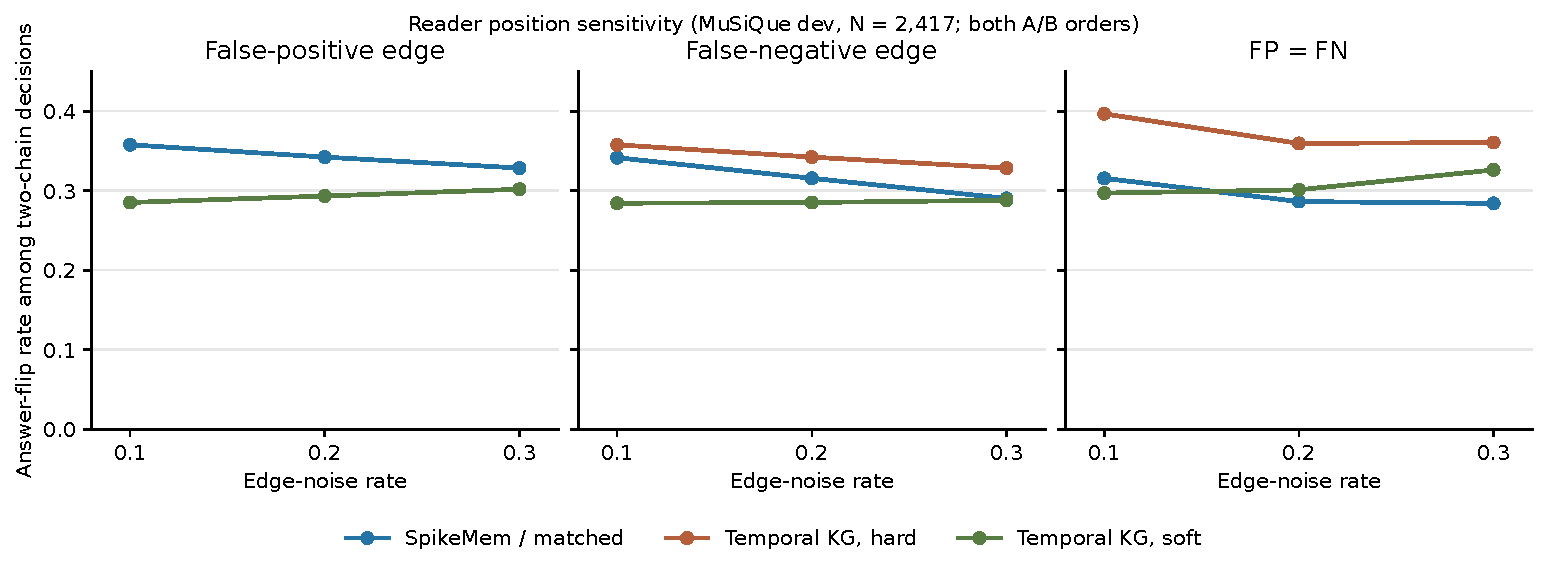
\includegraphics[width=\columnwidth]{fig4_order_flip.pdf}
\caption{Fraction of two-chain reader decisions whose answer changes when the presentation order is
reversed, across settings and methods. Every change is the reader selecting the first-presented chain
in both orders.}
\label{fig:flip}
\end{figure}

Figure~\ref{fig:flip} shows the order-flip rate across settings. Over the $14{,}292$ deduplicated
two-chain decisions of our full-dev runs, $4{,}314$ ($30.2\%$) change answer under reversal. Among the
$13{,}727$ decisions with a gold chain present, $9{,}820$ are correct in both orders, $3{,}907$ are
order-dependent, and none selects the same wrong answer in both orders. A fixed presentation order can
therefore bias a comparison between memories in either direction, which is why all numbers in this
paper are order-balanced.

\section{Abstention}
\label{sec:abstain}

On the full-dev \textsc{fp}$=0.3$ soft-invalidation run, $72$ two-chain cases contain no correct
answer in either candidate; the reader abstains in none of them, in either order. The same holds for
$20$ cases under \textsc{fn}$=0.3$ and $72$ under the diagonal setting. This agrees with prior findings
that offering an abstention option does not by itself produce abstention.

\end{document}
